\section{Domínio de aplicação do sistema}

Com o diagrama abaixo representado (Figura~\ref{fig:2}) é possível visualizar todos os atores do \textit{software} e as suas ações, assim como os sistemas envolvidos na aplicação e as funções.
Destes é possível identificar que este \textit{software} contém três atores principais, o Utilizador que é um utilizador sem sessão iniciada, o Técnico, um utilizador com sessão iniciada, já a Empresa é uma empresa cliente da Motorline. Também é possível visualizar os diferentes sistemas integrados no projeto, como Servidor Motorline onde serão obtidas informações do catálogo de produtos, Servidor \textit{Install \& Go} onde estão todas as funções de suporte ao \textit{software}, o Servidor de Imagens onde serão guardadas todas as imagens da aplicação e por fim o Servidor de \textit{Email} que enviará \textit{email} com o código de validação de conta para os clientes assim que se registarem no \textit{software}.

\begin{figure}[htb]
    \centering
    
    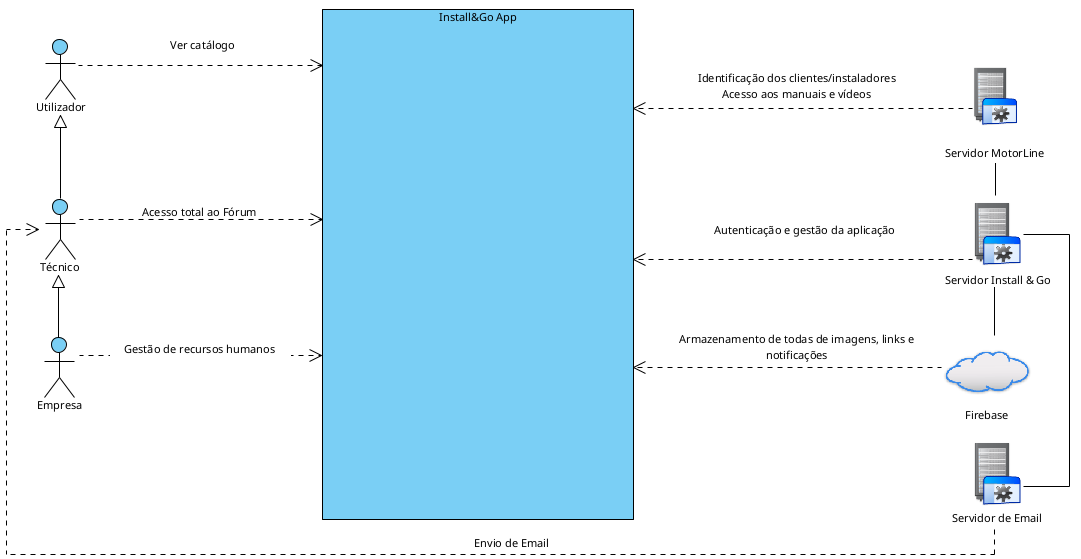
\includegraphics[width=\textwidth]{images/diagramas/diagrama_contexto.png}
    \caption{Diagrama de contexto da aplicação}
    \label{fig:2}
\end{figure}